\documentclass[../main-sheet.tex]{subfiles}
\usepackage{../style}
\graphicspath{ {../img/} }
\backgroundsetup{contents={}}
\begin{document}
\chapter{Graphical Theory For Solution of ODE}
\section{Integral Curves or Solution Curves}
Let
\begin{equation}
    \ddx{y}=f(x,y) \label{eq:i1}
\end{equation}
be a first order ordinary differential equation, then the graph of the explicit solution of \eqref{eq:i1} in the \(xy\) plane are called integral curves or solution curves.
\section{Line Element}
Let
\begin{equation}
    \ddx{y}=f(x,y) \label{eq:l1}
\end{equation}
be a first order ordinary differential equation, then a short segment of the tangent line through the point \((a,b)\) and with the slope \(f(a,b)\) is called the line element.
\subsection{Example of Line Element}
Suppose
\begin{equation}
    y'=2x+y\label{eq:le1}
\end{equation}
be an ordinary differential equation.\\
Here, \(f(x,y)=2x+y\)\\
The slope of \eqref{eq:le1} at \((1,2)\) is 4.\\
Thus, through \((1,2)\) we can draw short line \(AB\) with an inclination \(\approx 76^{\circ}\).
\begin{figure}[H]
    \centering
    \begin{tikzpicture}
        \begin{axis}[anchor=origin,axis lines=middle,xmax=4,xmin=-4,ymax=4,ymin=-4,ylabel style={above},
                ylabel={$y$},
                xlabel style={right},
                xlabel={$x$}]
            \addplot[thick,domain=1:1.25] (x,4*x-2);
            \addplot[black] coordinates {(1,2) (1.75,2)};
            \draw (1.75,2) coordinate (A) -- (1,2) coordinate (B)
            -- (1.05,2.2) coordinate (C)
            pic [draw,thick,angle radius=.4cm] {angle = A--B--C};
            \node at (1,1.5) {$(1,2)$};
            \node[left] at (1,2) {$A$};
            \node[left] at (1.05,3) {$B$};
            \node[left] at (2.4,2.5) {$76^{\circ}$};
        \end{axis}
    \end{tikzpicture}
\end{figure}
Here, \(AB\) is line Element at \((1,2)\).
\subsection{Line Element Configuration}
If we draw a large number of line element for a large number of points then we obtain a configuration called line element configuration.
\section{Direction Field}
The totality of the line element together with the corresponding directions constitute a field which is called direction field of the differential equation.

\section{Graphical Method}
A procedure which yields the line element configuration of the direction field of a differential equation is called the graphical method. It provides approximate graphs of solution curves.

\begin{prob}
    Construct a line element configuration (direction field) of the differential equation \(y'=\frac{y}{x}\) and sketch the several integral curves.
\end{prob}
\begin{soln}
    We have
    \begin{equation}
        y'=\frac{y}{x}\label{eq:p1.1}
    \end{equation}
    Here, the slope of the differential equation is
    \[m=\tan \theta =\frac{y}{x}\]
    The slope of the approximate integral curves of \eqref{eq:p1.1} are calculated at some selected points are given below.
    \begin{table}[H]
        \centering
        \newcolumntype{A}{>{$\displaystyle }c<{$}}
        \begin{tabular}{|A|A|A|A|A|A|A|A|A|A|A|A|A|}
            \hline
            x      & -1         & 1          & -2         & 2          & 1           & -1          & 2           & 3          & 3           & -2          & -3          & -3          \\\hline
            y      & -1         & 1          & -2         & 2          & -1          & 1           & -2          & 3          & -3          & 2           & 3           & -3          \\\hline
            m      & 1          & 1          & 1          & 1          & -1          & -1          & -1          & 1          & -1          & -1          & -1          & -1          \\\hline
            \theta & 45^{\circ} & 45^{\circ} & 45^{\circ} & 45^{\circ} & -45^{\circ} & -45^{\circ} & -45^{\circ} & 45^{\circ} & -45^{\circ} & -45^{\circ} & -45^{\circ} & -45^{\circ} \\\hline
        \end{tabular}
    \end{table}
    Now construct the line element at the selected points and sketch several smooth curves.
    \begin{figure}[H]
        \centering
        \begin{tikzpicture}
            \begin{axis}[anchor=origin,axis lines=middle,xmax=4,xmin=-4,ymax=4,ymin=-4,ticks=none,xlabel={$x$},ylabel={$y$},xlabel style={right},ylabel style={above}]
                \addplot[thick,domain=-3:3,-latex] (x,x);
                \addplot[thick,domain=-3:3,-latex] (x,-x);
                \node at (1.2,-0.5) {$(0,0)$};
            \end{axis}
        \end{tikzpicture}
    \end{figure}
    We observe that the integral curves represent a family of straight line passing through the origin.
\end{soln}
\begin{prob}
    Construct a line element configuration (direction field) of the differential equation \(y'=-\frac{x}{y}\) and sketch several integral curves.
\end{prob}
\begin{soln}
    We have
    \begin{equation}
        y'=-\frac{x}{y}\label{eq:p2.1}
    \end{equation}
    Here, the slope of the differential equation is
    \[m=\tan \theta =-\frac{x}{y}\]
    The slope of the approximate integral curves of \eqref{eq:p2.1} are calculated at some selected points are given below.
    \begin{table}[H]
        \centering
        \newcolumntype{A}{>{$\displaystyle }c<{$}}
        \begin{tabular}{|A|A|A|A|A|A|A|A|A|A|A|A|A|}
            \hline
            x      & 1         & -1          & -1         & 2          & -2           & -2          & 0           & 0          & 0           & 0          & 3          & -3          \\\hline
            y      & 1         & 1          & -1        & 2          & 2          & -2           & 1          & 2          & -2          & -1           & 3           & 3          \\\hline
            m      & -1          & 1          & -1          & -1          & 1          & -1          & 0          & 0          & 0          & 0          & -1          & 1          \\\hline
            \theta & -45^{\circ} & 45^{\circ} & -45^{\circ} & -45^{\circ} & 45^{\circ} & -45^{\circ} & 0^{\circ} & 0^{\circ} & 0^{\circ} & 0^{\circ} & -45^{\circ} & 45^{\circ} \\\hline
        \end{tabular}
    \end{table}
    We now construct the line element at the selected points and sketch several integral curves.
    \begin{figure}[H]
        \centering
            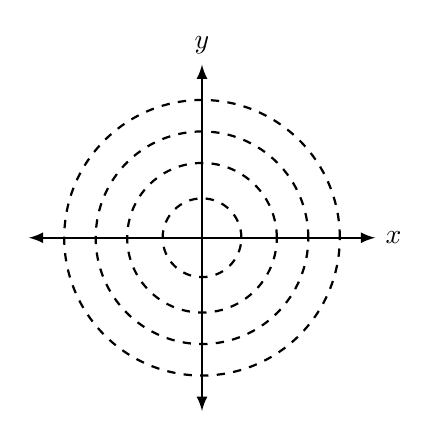
\begin{tikzpicture}
                \draw[thick,latex-latex] (-2.2,0)--(2.2,0)node[right] {$x$};
                \draw[thick,latex-latex] (0,-2.2)--(0,2.2)node[above] {$y$};
                \draw[thick, dashed] (0,0) circle (.5);
                \draw[thick, dashed] (0,0) circle (.95);
                \draw[thick, dashed] (0,0) circle (1.35);
                \draw[thick, dashed] (0,0) circle (1.75);
                \end{tikzpicture}
    \end{figure}
    We observe that the integral curves represent a family of circles which are centered as \((0,0)\).
\end{soln}
\section{Method of Isoclines}
Let us consider the differential equation
\begin{equation}
    \ddx{y}=f(x,y) \label{eq:iso1}
\end{equation}
A curve along which the slope \(f(x,y)\) has a constant value \(c\), is called a isocline of the differential equation \eqref{eq:iso1} are curves \(f(x,y)=c\) for different values of \(c\).
\begin{prob}
    Employ the method of isocline to sketch the several approximate integral curves of \(y'=3x-y\)
\end{prob}
\begin{soln}
    \begin{equation}
        \ddx{y}=3x-y\label{eq:piso1.1}
    \end{equation}
    and the isocline of \eqref{eq:piso1.1} is given by 
    \begin{align}
        &3x-y=c\notag\\
        \Rightarrow\,&y=3x-c\label{eq:piso1.2}
    \end{align}
    For different values of \(c\) \eqref{eq:piso1.2} represent a family of straight line.\\
    We construct the line \eqref{eq:piso1.2} for \(c=0,\pm1,\pm2,\pm3,\dots\) etc.\\
    On each of these lines we then construct a number of line elements having the approximate inclinations \(\tan^{-1}c\).
    \begin{align*}
        \text{When } & c=0,  & \text{ then } & y=3x,   &&\theta=\tan^{-1}c=0^{\circ}\\
        \text{When } & c=1,  & \text{ then } & y=3x-1, &&\theta=\tan^{-1}c=45^{\circ}\\
        \text{When } & c=-1, & \text{ then } & y=3x+1, &&\theta=\tan^{-1}c=-45^{\circ}\\
        \text{When } & c=2,  & \text{ then } & y=3x-2, &&\theta=\tan^{-1}c=63.43^{\circ}\\
        \text{When } & c=-2, & \text{ then } & y=3x+2, &&\theta=\tan^{-1}c=-63.43^{\circ}
    \end{align*}
    \begin{figure}[H]
        \centering
        \import{../tikz/}{iso-1.tikz}
    \end{figure}
    Finally we draw several smooth curves. These smooth curves represent the approximate integral curves of \eqref{eq:piso1.1}
\end{soln}
\begin{prob}
    Employ the method of isocline to sketch the several approximate integral curves of \(y'=2x+y\)
\end{prob}
\begin{soln}
    \begin{equation}
        \ddx{y}=2x+y\label{eq:piso2.1}
    \end{equation}
    The isocline of \eqref{eq:piso2.1} is given by 
    \begin{equation}
        2x+y=c\label{eq:piso2.2}
    \end{equation}
    For different values of \(c\) \eqref{eq:piso2.2} represent a family of straight line.\\
    We construct the line \eqref{eq:piso2.2} for \(c=0,\pm1,\pm2,\pm3,\dots\) etc.\\
    On each of these lines we then construct a number of line elements having the approximate inclinations \(\tan^{-1}c\).\\
    \begin{align*}
        \text{When } & c=0,  & \text{ then } & y=-2x,   &&\theta=0^{\circ}\\
        \text{When } & c=1,  & \text{ then } & 2x+y=1, &&\theta=45^{\circ}\\
        \text{When } & c=-1, & \text{ then } & 2x+y=-1, &&\theta=-45^{\circ}\\
        \text{When } & c=2,  & \text{ then } & 2x+y=2, &&\theta=63.43^{\circ}\\
        \text{When } & c=-2, & \text{ then } & 2x+y=-2, &&\theta=-63.43^{\circ}
    \end{align*}
    \begin{figure}[H]
        \centering
        \import{../tikz/}{iso-2.tikz}
    \end{figure}
    Finally we draw several smooth curves. These smooth curves represent the approximate integral curves of \eqref{eq:piso2.1}
\end{soln}
\begin{prob}
    Employ the method of isocline to sketch the several approximate integral curves of \(y'=\frac{y-x}{y+x}\)
\end{prob}
\begin{soln}
    \begin{equation}
        \ddx{y}=\frac{y-x}{y+x}\label{eq:piso3.1}
    \end{equation}
    The isocline of \eqref{eq:piso3.1} is given by 
    \begin{align}
        &\frac{y-x}{y+x}=c\notag\\
        \Rightarrow\,&y-x=cy+cx\notag\\
        \Rightarrow\,&(1+c)x=(1-c)y\notag\\
        \Rightarrow\,&y=\frac{1+c}{1-c}x\label{eq:piso3.2}
    \end{align}
    
    For different values of \(c\) \eqref{eq:piso3.2} represent a family of straight line passing through origin.\\
    We construct the line \eqref{eq:piso3.2} for \(c=0,\pm1,\pm2,\pm3,\dots\) etc.\\
    On each of these lines we then construct a number of line elements having the approximate inclinations \(\tan^{-1}c\).\\
    \begin{align*}
        \text{When } & c=0,  & \text{ then } & y=x,   &&\theta=0^{\circ}\\
        \text{When } & c=1,  & \text{ then } & x=0, &&\theta=45^{\circ}\\
        \text{When } & c=-1, & \text{ then } & y=0, &&\theta=-45^{\circ}\\
        \text{When } & c=2,  & \text{ then } & y=-3x, &&\theta=63.43^{\circ}\\
        \text{When } & c=-2, & \text{ then } & y=-\frac{1}{3}x, &&\theta=-63.43^{\circ}\\
        \text{When } & c=\infty, & \text{ then } & y=-x, &&\theta=90^{\circ}
    \end{align*}
    \begin{figure}[H]
        \centering
        \import{../tikz/}{iso-3.tikz}
    \end{figure}
    Finally we draw several smooth curves. These smooth curves represent the approximate integral curves of \eqref{eq:piso3.1}
\end{soln}
\begin{prob}
    Employ the method of isocline to sketch the several approximate integral curves of \(y'=\frac{3x-y}{x+y}\)
\end{prob}
\begin{soln}
    \begin{equation}
        \ddx{y}=\frac{3x-y}{x+y}\label{eq:piso4.1}
    \end{equation}
    The isocline of \eqref{eq:piso4.1} is given by 
    \begin{align}
        &\frac{3x-y}{x+y}=c\notag\\
        \Rightarrow\,&3x-y=cy+cx\notag\\
        \Rightarrow\,&(3-c)x=(c+1)y\notag\\
        \Rightarrow\,&y=\frac{3-c}{c+1}x\label{eq:piso4.2}
    \end{align}
    
    For different values of \(c\) \eqref{eq:piso4.2} represent a family of straight line passing through origin.\\
    We construct the line \eqref{eq:piso4.2} for \(c=0,\pm1,\pm2,\pm3,\dots\) etc.\\
    On each of these lines we then construct a number of line elements having the approximate inclinations \(\tan^{-1}c\).\\
    \begin{align*}
        \text{When } & c=0,  & \text{ then } & y=3x,   &&\theta=0^{\circ}\\
        \text{When } & c=1,  & \text{ then } & y=x, &&\theta=45^{\circ}\\
        \text{When } & c=-1, & \text{ then } & x=0, &&\theta=-45^{\circ}\\
        \text{When } & c=2,  & \text{ then } & y=\frac{1}{3}x, &&\theta=63.43^{\circ}\\
        \text{When } & c=-2, & \text{ then } & y=-5x, &&\theta=-63.43^{\circ}\\
        \text{When } & c=3, & \text{ then } & y=0, &&\theta=71.57^{\circ}\\
        \text{When } & c=-3, & \text{ then } & y=-3x, &&\theta=-71.57^{\circ}\\
        \text{When } & c=\infty, & \text{ then } & y=-x, &&\theta=90^{\circ}
    \end{align*}
    \begin{figure}[H]
        \centering
        \import{../tikz/}{iso-4.tikz}
    \end{figure}
    Finally we draw several smooth curves. These smooth curves represent the approximate integral curves of \eqref{eq:piso4.1}
\end{soln}
\end{document}